\section{Experiments}
% (recommended size: 1.5 pages)
	In this section, we will first describe the realistic simulation of clients connecting/disconnecting from the server, a requirement of the customer WantGame BV. After that, we first discuss our experimental setup. Finally, we describe the experiments we have conducted on FDDG and the outcome of these experiments.
	
\subsection{Simulation of connecting/disconnecting clients}
\label{subsec:simulation_clients}
A requirement of our game is that a realistic game trace should be used to simulate the behavior of clients connecting and disconnecting to and from the server.
A potential data set with game traces we can use is described in the paper of Guo et al. \cite{guo2012game}.
Here, the design of the GTA (Game Trace Archive) is explained and possible applications of the data are discussed.
Amongst the genres of the analyzed games are Massively Multiplayer Online Role-Playing Game (MMORPGs), board games and Real-time Strategy (RTS) games. 
Since our games closely resembles a MMORPG, we decided to use the WoWAH game trace \cite{lee2011world}.
This game trace archive contains data about 91065 players during 1107 days. The dataset is available as a free download on their website\footnote{http://mmnet.iis.sinica.edu.tw/dl/wowah/}.
We gathered data about the number of online players during 24 hours. 
A visual representation of the amount of online avatars in the game trace can be found in Figure \ref{fig:online_players_plot}. As we see, the number of online players is minimal during the morning and maximal around midnight.

\begin{figure}[h!]
  \centering
    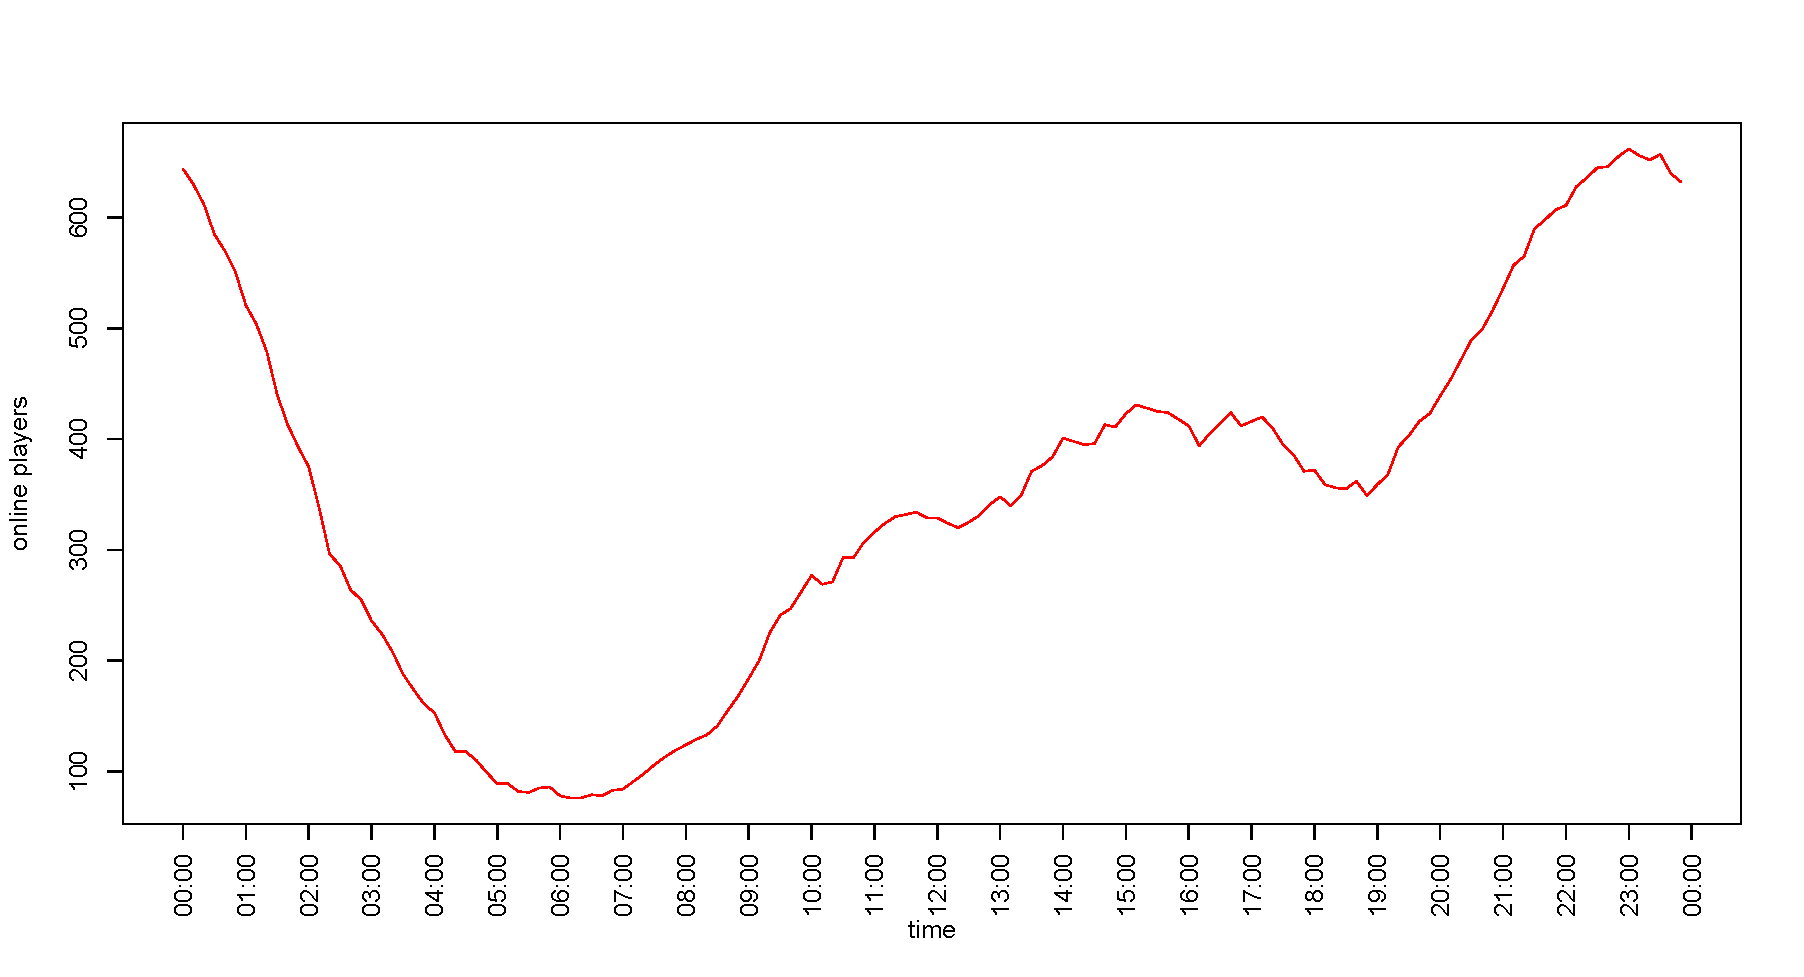
\includegraphics[width=\textwidth]{images/online_players_plot}
    
  \caption{The number of online players during 24 hours (2007-07-14)}
  \label{fig:online_players_plot}
\end{figure}

We keep track of the number of players connecting and disconnecting during 10-minute time intervals.
We used that interval because in the WoWAH dataset, samples are taken every 10 minutes.
Using this data, we were able to create a realistic pattern of players connecting and disconnecting to and from the game.
A simulation file has been created, containing information about all events during 24 hours. This file can be used to actually run the simulation of connecting and disconnecting players.

\subsection{Experimental setup}
\label{subsec:experimental_setup}
% Describe the working environments (DAS-4, Amazon EC2,
% etc.), the general workload and monitoring tools and libraries, other tools and
% libraries you have used to implement and deploy your system, other tools and
% libraries used to conduct your experiments.

	To experiment with our game and see how it performs, we decided to simulate the game on the DAS-4 supercomputer.
	The common setup of our experiments consisted of 5 servers where each server runs on one of the DAS-4 nodes. Furthermore, we have two nodes with 50 client running on each node.
	By running the simulations on the DAS-4, we guaranteed that we tested in a truly distributed system where processes were running on physical different machines.
	The disadvantage of running our game on the DAS-4 is that we cannot see the GUI that allows for easier debugging and observation of the game state.
	Furthermore, we've developed our own message system that makes use of \emph{actions} to implement updates and acknowledgments.
	A simulation starts as soon as the first client joins the server. The game is then considered active and will run until either all players are dead or all dragons are slain.


\subsection{Experiments}
\label{subsec:experiments}
% Describe the experiments you have conducted to analyze each
% system feature, such as consistency, scalability, fault-tolerance, and
% performance. Analyze the results obtained for each system feature. Use one
% sub-section per experiment (or feature). In the analysis, also report:
% i. Service metrics of the experiment, such as runtime and response time of
% the service, etc.
% ii. (optional) Usage metrics and costs of the experiment.
	We ran experiments concerning the consistency, fault-tolerance and scalability of the game. Below are the results of the experiments conducted for each of these features. Moreover, we made an analysis of the number of messages in the game.

	\subsubsection{Consistency}
	\label{subsubsec:consistency}
		One of the properties of the game is that there is consistency amongst the servers.
		In order to test the consistency between the servers, we made use of the GUI and see whether two or more servers are synchronized and lead to the same end state.
		While testing the consistency, some minor bugs were found that have led to an inconsistent game state. These were fixed during the experiments.
		We tested the consistency with several setups. For example, we made dragons much stronger than players to see the impact of players dying very fast after they are spawned.
		Moreover, we manually tested what happened when players can easily kill dragons.
		We were not able to find inconsistencies while manually testing. We have concluded that the games we simulated end in the same final state on all servers.
		
	\subsubsection{Fault-tolerant}
	\label{subsubsec:fault-tolerant}
		To test fault-tolerance, the following scenarios are considered:
		\begin{enumerate}
			\item During simulations, some some client nodes are killed. The servers should then remove the players from the field and continue the game.
			\item During the simulation, one server is killed. Clients should connect to another server in this case.
		\end{enumerate}
		
		More information about the design of fault tolerance in our system can be found in section \ref{subsubsec:client_server_crashes}. If a client crashed, the server should notice that after two failed heartbeats to this client. During our simulations, the event that a server sends two failed heartbeats to the client is logged. Using the GUI, it is possible to determine whether the player is really removed from the server. This turned out to be the case if clients are crashed on purpose. The servers remove the disconnected player from the field and continue the game.\\
		When a server fails, clients should immediately reconnect to one of the other available servers. When killing a server, we noticed that the clients connected to this server, were trying to select another server that is still available. Only if all servers are down, clients will stop trying to connect to one of the servers.
		
	\subsubsection{Scalability}
	\label{subsubsec:scalability}
		The minimum requirements of running 5 servers, 100 clients and 20 dragons were easily fulfilled. We therefore decided to try 10 servers, 200 clients and 40 dragons (twice as much for every parameter). The results were ...
		
	\subsubsection{Message complexity of the system}
	\label{subsubsec:nummessages}
		The chosen consistency model in the game has great impact on the number of messages between servers and clients. 
		In this subsection, an analysis of the total number of messages in the system is performed and simulations of clients and servers are performed to determine the total number of required messages.\\
		First, we take a look at the number of messages required for a client to perform an action. 
		A client performing an action, sends this action to the server it is connected to. 
		The server sends this request to all other servers and these servers respond with an acknowledgment if the action is valid. 
		Finally, the server let all other servers know this action can be performed. 
		The action is then performed and send to all clients. 
		More information about this process can be found in section \ref{subsubsec:clients_actions}. 
		The total number of messages required for one action can be described by the following formula ($ n $ is the total number of messages, $ s $ is the number of servers, $ c $ is the number of clients):
		$$ n = 3(s - 1) + c + 1 $$
		The formula above excluded heartbeat messages sent between clients and servers.
		We can use this formula to make an approximation of the amount of messages that has to be sent between the servers and clients. 
		Suppose $ s = 5 $ and $ c = 100 $. 
		If every client performs an action every second, a total of 678.000 messages to be exchanged or about 6780 messages for every client. 
		This number can be reduced by switching to another model for consistency.\\
		To gain more insight in the number of messages, we ran the setup with 5 servers and 20 dragons. 
		We had two runs, one with 50 clients and one with 100 clients. 
		In both cases, it took around one minute to finish the game (in both games, all players were killed). 
		With 50 clients, the total number of messages was around 5600 from the beginning to the end of the game. 
		With 100 clients, a total of 14900 messages between servers and clients are exchanged. 
		The fact that this number is way below the approximated number of messages in the system can be explained by the fact that not all clients were active during the total duration of the game. 
		Moreover, players that have died during the game, have no chance of performing actions. We also noticed that the number of messages sent by a server to clients are about 2.5 times larger than the number of messages to other servers.\\
		The final analysis discussed here is the number of heartbeats between clients and servers. 
		With five servers, each server received and sent around 150 heartbeats. 
		The total number of heartbeats sent to clients is for each server around 105. 
		We can conclude that these numbers are not significant and the main cause of messages in the system is caused by actions in the game.
